\section{Circuito RLC}

\subsection{Conceitos}

Um circuito RLC é um circuito elétrico composto de um resistor (R), um indutor (L), e um capacitor (C), conectados em série ou em paralelo.

É um \textbf{circuito de 2° ordem}, pois qualquer tensão ou corrente nele pode ser descrita por uma equação diferencial de segunda ordem.

\begin{figure}[H]
	\centering
	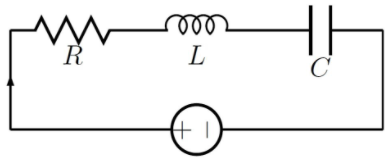
\includegraphics[width=0.8\textwidth]{./Imagens/RLC/rlc1.png} 
	\caption{Desenho esquemático de um circuito RLC}
	\label{fig:RLC1}
\end{figure}

\subsubsection{Indutor}

Um indutor é um componente eletrônico passivo capaz de armazenar energia elétrica na forma de \textbf{energia magnética}. Basicamente, é constituído de um condutor que é enrolado em uma bobina, e quando a eletricidade flui para a bobina da esquerda para a direita, isso gera um campo magnético cujo sentido pode ser obtido pela regra da mão direita.

O indutor no esquema é usado para representar as características físicas do circuito. Ele representa a "inércia elétrica" do circuito: à medida que a corrente flui no circuito ela gera um campo magnético ao redor do condutor. A intensidade do campo depende da magnitude da corrente e segue quaisquer mudanças na corrente. Pela lei da indução de Faraday, essa mudança no campo magnético induz uma força eletromotriz nos condutores, processo chamado de \textbf{indução eletromagnética}. Esta tensão induzida, por sua vez, pela lei de Faraday-Neumann-Lenz gera uma tensão no circuito que é oposto à tensão que está gerando o campo magnético (V1). Esta é a razão porque a corrente no circuito não salta imediatamente para o seu valor total de V/R dado pela lei de Ohm. A corrente acabará por atingir o valor V/R após um período infinito de tempo, mas para fins práticos consideramos um tempo menor.

\subsubsection{Capacitor}

Similarmente aos indutores, os capacitores também armazenam energia, porém, na forma eletrostástica. 

\subsubsection{Frequência de ressonância}

A frequência natural ou de ressonância sem carga de um circuito RLC (em radianos por segundo) é:

\[\large \omega _{o} = \frac{1}{\sqrt{LC}}\]

Em Hertz é:

\[\large f_{o} = \frac{\omega _{o}}{2\pi} = \frac{1}{2\pi\sqrt{LC}}\]

\subsubsection{Impedância}

A energia aplicada por segundo a um circuito de corrente alternada (potência do circuito) é destinada a vencer as três dificuldades presentes no mesmo: a resistência efetiva, a reatância indutiva e a reatância capacitiva.

A impedância é a resistência (ou oposição) de um circuito à corrente alternada e sua unidade de medida é o "ohm". Para calculá-la, deve-se conhecer o valor de todos os resistores e a reatância de todos indutores e capacitores do circuito.

\subsection{Equação do circuito RLC}

Quando uma resistência está presente, a energia eletromagnética total U do circuito não é constante mas diminui com o tempo na medida em que essa energia é dissipada na forma de calor pelo resistor.

A energia total é dada pela soma das energias magnética do indutor ($U_{B}$) e energia elétrica do capacitor ($U_{E}$):

\[\large U = U_{b} + U_{E} = \frac{1}{2}Li^2+\frac{q^2}{2C}\]

onde $\large \frac{dU}{dt} = -i^2R$ representa a taxa de perda de energia por calor.

Se derivarmos a equação da energia em relação à t, obteremos:

\[\large \frac{dU}{dt} = Li\frac{di}{dt} + \frac{q}{c}\frac{dq}{dt} = -i^2R\]

Substituindo i por $\frac{dq}{dt}$ e $\frac{di}{dt}$ por $\frac{d^2q}{dt^2}$ obtemos a equação diferencial que descreve as oscilações amortecidas de circuitos RLC:

\[\large L\frac{d^2q}{dt^2}+R\frac{dq}{dt}+\frac{1}{C}q = 0\]

A solução geral dessa equação é:

\[\large q = Qe^{-Rt/2L}cos(\omega't + \phi)\]

na qual $\large \omega' = \sqrt{\omega^2-(R/2L)^2}$ e $\omega$ é a frequência de ressonância do circuito.

O gráfico da corrente em função do tempo mostra que a amplitude da corrente decrescente exponencialmente com o tempo:

\begin{minted}{python}
import matplotlib.pyplot as plt
import numpy as np
import math

fig, ax = plt.subplots(figsize = (8,5))

t = np.linspace(0,0.1,500)
L = 70*10**(-3)
C = 2.5*10**(-6)
# Ohms
R = 10
fi = 0
Q = 1

w = 1/(math.sqrt(L*C))
wl = np.sqrt(w**2-(R/(2*L))**2)
#print(wl)
q = Q*np.exp(-R*t/(2*L))*np.cos(wl*t+fi)
ax.plot(t,q)

#Altera o tamanho do nome dos eixos
plt.xlabel('tempo (t)', fontsize=15) 
plt.ylabel('q (carga)', fontsize=15)

plt.show()
\end{minted}

\begin{figure}[H]
	\centering
	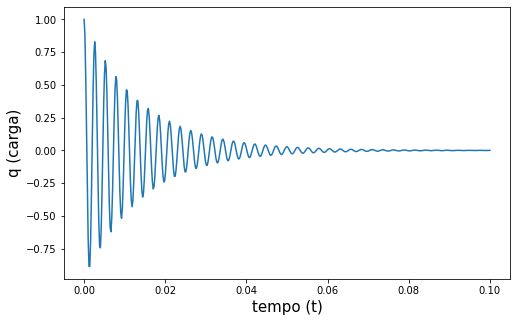
\includegraphics[width=0.8\textwidth]{./Imagens/RLC/rlc2.png} 
	\caption{Carga x tempo}
	\label{fig:RLC2}
\end{figure}

\section{Oscilações forçadas}

Oscilações forçadas são aquelas que ocorrem quando o circuito RLC é submetido à uma fonte externa de força eletromotriz alternada. Agora, essa força eletromotriz irá variar com um frequência angular controlada $\omega$ (chamada de propulsora), de acordo com a equação abaixo:

\[\large \xi = \xi _{m}sen(\omega \cdot t)\]

Onde $\xi_{m}$ é a amplitude da fem. As oscilações da carga, corrente e diferença de potencial no circuito são chamadas de oscilações forçadas.

A frequência natural de vibração do sistema será:

\[\large \omega_{0} = \frac{1}{\sqrt{LC}}\]

A figura abaixo compara o sistema eletromagnético oscilante a um sistema mecânico correspondente:

\begin{itemize}
\item O vibrador V que impõe uma força externa alternada corresponde ao gerador G que impõe uma fem alternada. 
\item O capacitor é análogo à mola, uma vez que ele, como a mola, armazena energia: a mola na forma de energia potencial elástica, e o capacitor na forma de energia potencial elétrica.
\item A massa mede a inércia, determinando a intensidade da força necessária para produzir no objeto a aceleração desejada; a indutância, de modo semelhante, mede o grau de dificuldade em alterar a corrente, determinando a força eletromotriz necessária para produzir no indutor o valor da corrente desejada.
\item Por fim, a resistência em um circuito elétrico é responsável pela dissipação de energia sob a forma de calor da mesma forma que o atrito é responsável pela dissipação da energia em um sistema mecânico, também sob a forma de calor.
\end{itemize}

\begin{figure}[H]
	\centering
	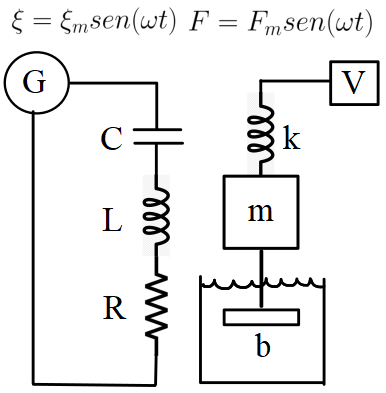
\includegraphics[width=0.5\textwidth]{./Imagens/RLC/rlc3.png} 
	\caption{Comparação de sistemas}
	\label{fig:RLC3}
\end{figure}

\subsubsection{Aplitude da corrente}

A amplitude da corrente em um circuito RLC em função da força eletromotriz senoidal aplicada, frequência angular de excitação $\omega_{d}$ e do valor da indutância (L) e capacitância (C) é:

\[\large I = \frac{\xi_{m}}{\sqrt{R^2+(\omega_{d}L-1/\omega_{d}C)^2}}\]

A amplitude será máxima quando a frequência $\omega_{d}$ se iguala à frequência natural de vibração $\omega_{n}$. A figura abaixo mostra as amplitudes para diversos valores de resistência. Em todos os casos, os circuitos RLC série que diferem apenas quanto ao valor de R e os valores máximos de suas amplitudes são inversamente proporcionais à R, assim como as suas larguras são proporcionais à R.

\begin{minted}{python}
	
import matplotlib.pyplot as plt
import numpy as np
import math

# fig, ax = plt.subplots(figsize = (10,8))

L = 4*10**(-3)
C = 2.5*10**(-6)
fem = 10
# frequência natural
wn = 1/(math.sqrt(L*C))
print(wn)
wd = np.linspace(0.01,2*wn,500)

def amp(R, wd, L, C, fem):
I = fem/(np.sqrt(R**2+(wd*L-1/(wd*C))**2)) 
return I

plt.figure(figsize=(10,5))
plt.plot(wd/wn,amp(5,wd, L, C, fem), color="blue", 
label='5')
plt.plot(wd/wn,amp(10,wd, L, C, fem), color="red", 
label='10')
plt.plot(wd/wn,amp(20,wd, L, C, fem), color="pink", 
label='20')
plt.axvline(1, color='black', linewidth=0.5)
plt.suptitle('Curvas de ressonância', fontsize=20)
#Altera o tamanho do nome dos eixos
plt.xlabel(r'$\frac{\omega_{d}}{\omega}$', fontsize=20) 
plt.ylabel('I (amplitude)', fontsize=20)
plt.grid()
plt.legend() #exibindo as legends
plt.show()
\end{minted}

\begin{figure}[H]
	\centering
	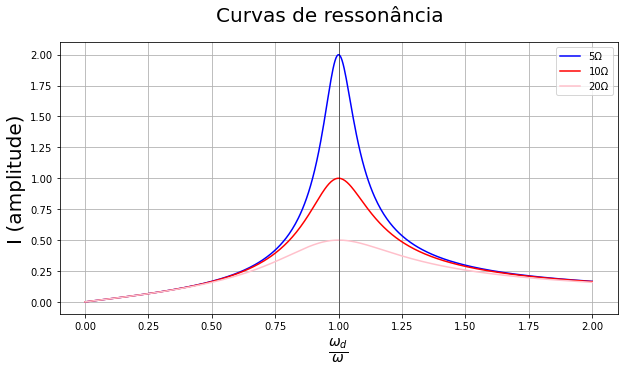
\includegraphics[width=0.8\textwidth]{./Imagens/RLC/rlc4.png} 
	\caption{Amplitude x frequência}
	\label{fig:RLC4}
\end{figure}

\section{Aplicações dos circuitos RLC}

\begin{itemize}
\item Receptores de rádio e aparelhos de televisão usam circuitos RLC para sintonização selecionando uma faixa estreita de frequência das ondas de rádio do ambiente. Nessa função, o circuito é frequentemente denominado circuito sintonizado. Um circuito RLC pode ser usado como filtro passa-banda, filtro passa-baixo ou filtro passa-alto. 
\item Os circuitos RLC são usados no sistema de ignição do automóvel para gerar uma tensão muito alta.
\item A resposta natural RLC cai em três categorias: superamortecido, criticamente amortecido e subamortecido, de forma semelhante como acontece em osciladores harmônicos amortecidos.
\end{itemize}